% Copyright (c) 2021 Tobias Briones. All rights reserved.
% SPDX-License-Identifier: CC-BY-4.0
%
% This file is part of https://github.com/tobiasbriones/
% cp-unah-mm700-agricultural-soil-sampling-for-data-analysis
%
% This source code is licensed under the Creative Commons Attribution 4.0
% International License found in the LICENSE-CC file in the root directory of
% this source tree or at https://spdx.org/licenses/CC-BY-4.0

\subsection{Muestreo Aleatorio Simple (MAS)}

Este tipo de muestreo es el más básico que se puede tomar y en base a él se desarrollan en gran medida los otros tipos de muestreo más compuestos. Las condiciones para que funciones son que las unidades de la población tenga igual probabilidad de ser escogidas. Los cálculos hechos para el MAS son también extendidos por otros métodos de muestreo, ya que al final siempre conllevan con algo de aleatoriedad.

\bigbreak

Es importante que el suelo sea homogéneo para realizar un muestreo simple aleatorio y probablemente también mezclar las muestras para obtener un compuesto. Para realizar el muestreo se pueden seguir varios patrones, a saber, zigzag, diagonal, etc.:

\begin{figure}[H]
    \centering
    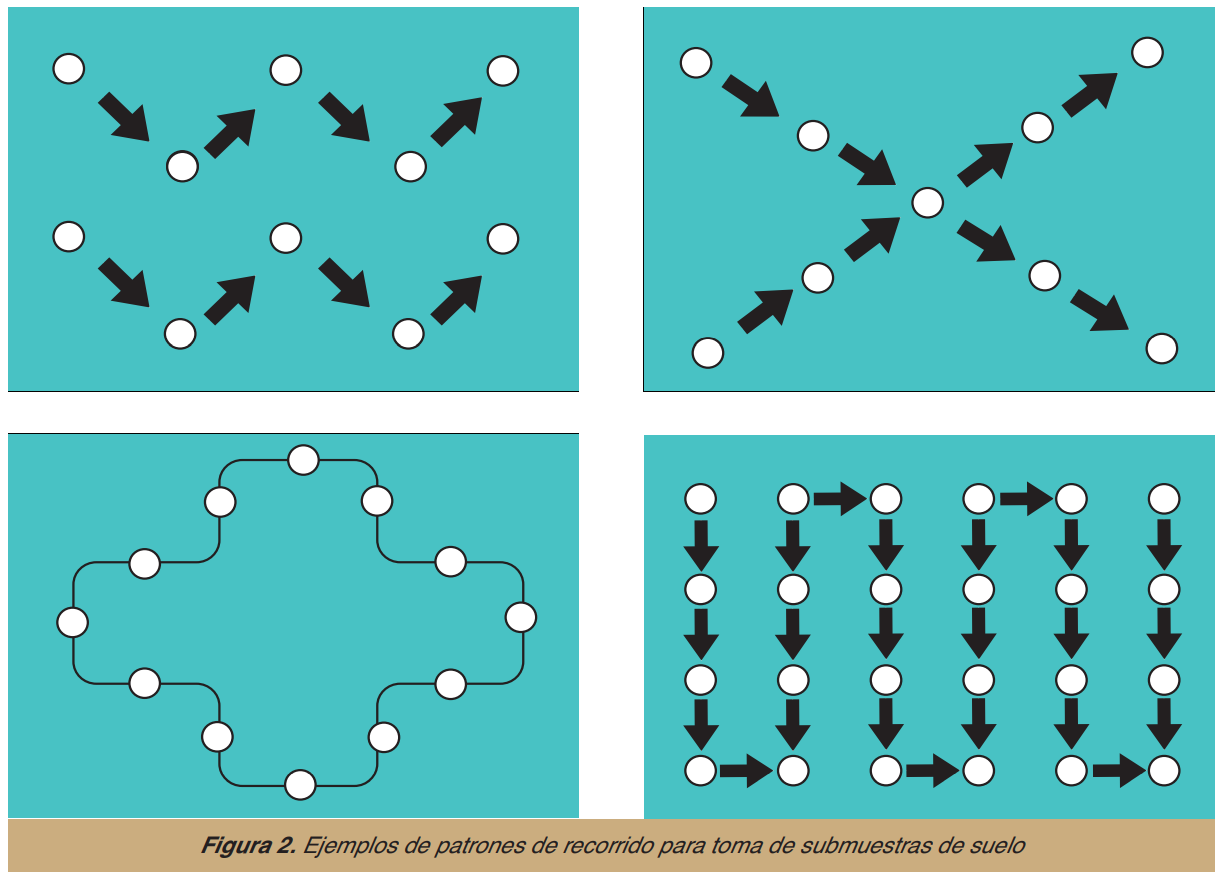
\includegraphics[width=0.3\paperwidth]{ref/sampling-patterns-srs.png}
    \caption{Patrones de muestreo para análisis de fertilidad de suelo}
    Fuente: Muestreo y análisis de suelos para diagnóstico de fertilidad \cite{lassaga-2011}
\end{figure}

Como se detalla más adelante, el terreno o lotes también se puede estratificar y realizar un MAS en cada estrato obtenido. El muestro sistemático por otra parte puede llegar a reducirse a un MAS o similar dado las condiciones apropiadas. Esto indica que el MAS es elemental para hacer otro tipo de diseño de muestreo.

\bigbreak

Estos son los resultados para los cálculos del MAS \cite{thompson-2012}:

\bigbreak
\textbf{Media de la población}

\bigbreak

$\overline{x}_U = \frac{1}{N}(x_1 + x_2 + ... + x_N) = \frac{1}{N} \sum \limits_{i=1}^N x_i$


\bigbreak
\textbf{Media de la muestra}

\bigbreak

$\overline{x} = \frac{1}{n}(x_1 + x_2 + ... + x_N) = \frac{1}{n} \sum \limits_{i=1}^n x_i$

\bigbreak

\textbf{Varianza de la población finita}

\bigbreak

En MAS, la varianza de la muestra $s^2$ es una estimación no-alineada de la varianza para la población finita

\bigbreak

$\sigma^2 = \frac{1}{N-1} \sum \limits_{i=1}^{N} (x_i - \overline{x}_U)^2$


\bigbreak
\textbf{Varianza de la muestra}

\bigbreak

$s^2 = \frac{1}{n-1} \sum \limits_{i=1}^n (x_i - \overline{x}_U)^2$


\bigbreak
\textbf{Total de la población}

\bigbreak

$t = \sum \limits_{i=1}^N x_i = N \overline{x}_U$
